\chapter{提案手法} % 一般の人がわかるレベルのアルゴリズム解説
\label{chap:approach}

\section{探索空間を限定する手法の提案}
\subsection{和了率の評価によるノードの展開}

本研究では、モンテカルロ法の探索空間が大きくなりすぎる問題に対して、特定のノードの牌姿に対する期待和了順目を次の節で説明する数理モデルを使って有望だと思われる手を探索するようにする。
1人麻雀において特定の牌姿の期待和了順目を途中で評価できることは、より有望な手を探索できる可能性がつながるため、UCB1などの評価値よりも手の有望さを評価する精度を上げることができると期待される。

\begin{figure}
 \centering
 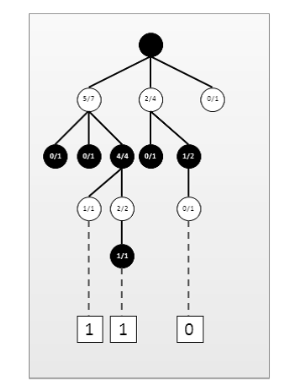
\includegraphics[keepaspectratio, scale=1.0,bb=0 0 304 387]
      {img/UCB.png}
 \caption{和了率評価を用いたモンテカルロ木探索}
 \label{monte2}
\end{figure}

\subsection{1人麻雀プレイヤにおける和了率の数理的評価}

国士氏の研究により、ある手牌における聴牌までの平均消費順目は、それぞれの変化での平均消費巡目のそれぞれの変化する確率での単純な平均で与えられることがわかっている。[3]すなわち、元の成功率がp、手変わりする確率がq,r、手変わり後の成功率がQ,Rならば、

その手の向聴が進むまでの平均消費巡目は

\begin{equation}
\label{kitai1}
\Large \displaystyle \frac {p\frac{1}{p} + q\frac{1}{Q} + r\frac{1}{R}}{p+q+r}
\end{equation}

と表される。

本論文ではこれを和了時までの式に拡張する。
まず、聴牌までの平均順目と聴牌後の和了までの平均順目の合計がすなわち全体の平均消費順目であることを証明する。
次に、それを合成した結果の数式がどうなるかを書く。

考察の結果このようになる。

\begin{equation}
\label{kitai2}
\Large \displaystyle \frac {p\frac{1}{p} + q\frac{1}{Q} + r\frac{1}{R}}{p+q+r} + 和了期待順目
\end{equation}

また、(現在の平均テンパイ巡目)=(次巡の平均テンパイ巡目)+1 であることから、
各ノードが手替わり率とテンパイ率を値として持つ深さ1の木構造で記述できる。 
したがって、同様に、n手先の手替わりまで考えると深さnの木構造で記述することができる。
nを大きくすることにより、精度の高い和了率を近似することが可能となる。

図Q
\begin{figure}
 \centering
 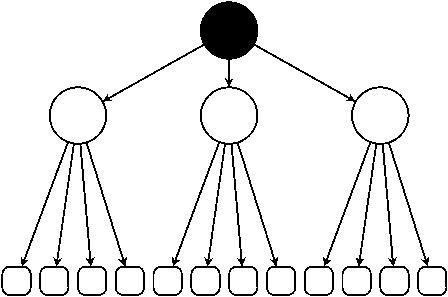
\includegraphics[keepaspectratio, scale=0.5,bb=0 0 500 281]
      {img/monte.jpg}
 \caption{図の説明}
 \label{ラベル名}
\end{figure}

本研究では、この式(3)をそれぞれの牌姿に当てはめ、その計算結果が高くなるようなノードを探索する。
これにより、従来の手法では何回も同じ牌姿の変化をシミュレートしなければいけない問題があったが、(3)式の評価によってその多くが削減できる。
したがって、この方法によって精度が高くなることが期待される。

\subsection{二向聴以下の牌姿に対してモンテカルロ法を適用する}

麻雀において、和了までの手順の中では、シャンテン数が小さい時点での選択が成績に影響を与えやすいことがわかっている\cite{gendai}
したがって、成績向上のためには和了系に近い部分において戦略を改善することが成績に影響を与えやすい事がわかる。

また、モンテカルロ法の問題点は、前述したとおり麻雀に適用すると探索空間が大きくなりすぎることが問題であった。しかしこれを和了系に近い部分に適用することで、
探索空間を小さく削減することができるため、適用することができるようになる。
本研究の手法である与えられた牌姿における和了率の近似式(3)を適用する際にも、シャンテン数が大きすぎる場合については正確に見積もることが難しいため、このような限定的な部分への適用が重要である。

本論文では二向聴以上の部分にこのモンテカルロ法を適用することで、従来の問題点を解決する。
